\chapter{Architectural Design}
  
\section{Overview}
In the following paragraphs we'll present a general overview of how the system is architected, with specific focus on the distinction between logically separated layers.

Specifically, myTaxiService has been envisioned from the ground up to be fully scalable and easily deployable on any number of servers. This characteristic is not only desirable, but actually fundamental for the system to fully accomplish the tasks it's been designed for. In order to guarantee this level of flexibility and modularity, we have settled for a system architecture that inherently enables a wide range of hardware configurations for all kinds of workloads.

The system architecture is thus logically organized in a set of interplaying software layers, whose detailed description is hereby presented.

\begin{figure}[H]
\centering
\makebox[\columnwidth]{\includegraphics[width=350pt,keepaspectratio]{pdfs/overall_architecture.pdf}}
\end{figure}
\vspace{5mm}
The lowest layer of the architecture is composed by the relational \textbf{Data-base Management System (DBMS)} that supports all data storage operations. This component fully supports ACID distributed transactions and is meant to be run inside a Demilitarized Zone (DMZ) which is separated from the rest of the system for security reasons.
In order to provide a higher level of abstraction to all components that need access to data and to be as platform agnostic as possible, the DBMS interface is not directly exposed to the classes that implements the business logic of the system. Instead, an intermediate \textbf{Data Layer} is responsible of performing queries on the DBMS while exposing a more flexible, customized interface to the upper layers.

The \textbf{Business Layer} implements all core functionalities of the system. In particular, all operations related to handling taxi requests and reservations, taxi availability and zone management are performed by components of this layer. Data is stored and retrieved using the APIs exposed by the Data Layer. Core functionalities are exposed to clients through a unified Application Façade that allows fine-grained tuning of which operations can be invoked from outside the central system.

The Business Layer also depends on an external \textbf{Mapping Service} for the implementation of reverse geocoding and waiting time estimation operations. This external service is directly invoked by classes of the Business Layer by using a public API provided by the Mapping Service itself. 

However, not every functionality exposed by the Application Façade may actually be made publicly available to every client. In principle, several levels of permissions could be offered to third parties while maintaining control over private APIs which should only be used by "official clients". Read-only reporting functionalities, for example, could be made available to any requesting party, while more critical operations could be offered only to selected developers after having verified certain requirements are satisfied. Furthermore, specific sets of APIs could be made available only to approved plugins and not be offered to remote services. For this reason, the \textbf{Services Layer} provides a comprehensive interface to all kinds of third party services and plugins by carefully defining which methods are available for remote and local invocation, what protocols should be followed for invoking them and what kind of messages can be exchanged between a remote component and the central system.

While locally invokable APIs are made available only to plugins, remotely invokable APIs are also offered to components living outside the perimeter of the central system. The \textbf{Message Broker and Notification System} is precisely concerned with guaranteeing an efficient and reliable communication channel with these remote entities by supporting message queues, publish/subscribe communications and dynamic, asynchronous event notifications.

The \textbf{Web Presentation Layer} is responsible for the implementation of the web application. It generates the dynamic web pages, offers them to the client via a web server, accepts requests and forwards them to the business layer by means of the communication layer and of the services layer. 

Finally, the \textbf{Mobile Applications} let users access the functionalities offered by the system on their smartphones and tablets in a native way. As for the web application, they interact with the central system using the communication layer and the services layer.
  
\section{High level components and their interactions}
The purpose of this section is to present the main components in which myTaxiService is divided and the relations between them.

In particular, it should be noted that the components discussed here are very abstract clusters of functionalities which do not directly map to any specific module in the final system. Instead, they are intended as an useful representation to show how the main functionalities of the system are grouped together and interact with each other. Further details on how these components are realized in the actual system will be discussed with greater depth in the Component view subsection.

A schematic representation of the component structure of the system is the following.
\begin{figure}[H]
\centering
\makebox[\columnwidth]{\includegraphics[width=450pt,keepaspectratio]{pdfs/overall_components.pdf}}
\end{figure}

The \textbf{Account Management} component is responsible for all operations related to user accounts. More specifically:
	\begin{itemize}
		\item It implements the passenger registration process
		\item It implements the login procedure for all users 
		\item It supports operations on existing accounts, including settings management and password retrieval operations
	\end{itemize}

The \textbf{Taxi Management System} is the single most important component in the system. It is responsible for:
	\begin{itemize}
		\item Maintaining the availability status of each taxi updated
		\item Managing the taxi queue associated with each zone in the city
		\item Accepting and managing taxi reservations
		\item Fulfilling taxi requests by selecting the first available taxi in the corresponding taxi zone  
	\end{itemize}
	
The \textbf{System Administration} component offers system configuration and monitoring functionalities. It enables the insertion, update and deletion of taxis and taxi drivers and the definition of the boundaries of the zones in which the city is divided. It also lets administrators perform queries to obtain system statistics including uptime, number of served requests per day and other key performance indicators. The user interface for interacting with this component is provided by a web application. 

The \textbf{Database Management System (DBMS)} is the component responsible for storing and retrieving data in a persistent, reliable way. It should be noted that this component will not be implemented from scratch; instead, a commercial solution will be used.

The \textbf{Data Access Utilities} component provides an abstraction layer to all those components that need to store data into the DBMS or retrieve data from it.

The \textbf{Mapping Service} component is provided by a third party and is accessed via a publicly available API. It is used to perform reverse geocoding and to compute the ETA of the taxi assigned to a certain request.

The \textbf{Remote Services Interfaces} component provides external applications and clients a way to invoke the services offered by the central system. Specifically, it implements a platform-independent, SOAP-based web service which exposes the full set of remotely invokable methods defined by the public API specification of myTaxiService.

The \textbf{Notification System} component implements an event-based mechanism to notify remote applications and clients of specific changes in the status of the central system. In particular, this is employed to let users known when the system has assigned a taxi to their reservation.

As for how the system can be accessed by its users, the \textbf{Taxi Driver Application} and the \textbf{Passenger Application} provide a way for taxi drivers and passenger respectively to interact with the system through their smartphones, while the \textbf{Passenger Web Application} allows passengers perform their operations through a web browser. Finally, administrators can access the system using the aforementioned \textbf{Administration Web Application}.



\section{Component view}
In this section, we'll provide a more detailed description of the most significant components that must be developed as part of myTaxiService.

It should be noted that, when multiple operations or tasks are managed by a certain sub-component, not all of them will be explicitly mentioned in this section. This is because, at this level of detail, we want to put the focus on the primary goal of every sub-component; an exhaustive description of the functionalities implemented by each sub-component will be presented in the Requirements Traceability section of this document. 

The first component that we'll examine is the \textbf{Taxi Management System}. As we already mentioned, this component is primarily responsible for all operations related to taxi management. Although it may appear to be an atomic component, it is in fact composed of three different sub-components, each of them dedicated to handling a specific subset of operations:
	\begin{itemize}
		\item The \textbf{Reservation Management} sub-component performs all the activities related to reservation handling. In particular, it is able to receive a request for a new reservation, store it into an internal data structure and periodically look for reservations that have come to expiration. Once such a reservation is found, it creates a request for it and transfers the computation to the Request Manager.
		\item The \textbf{Request Management} sub-component performs all the activities related to request handling. In particular, it is able to receive a new taxi request (either from an end user or from the reservation manager), retrieve the associated geographical coordinates through invocation of the Mapping Service API if the request only contains the meeting address, and use them to discover the zone from which the request is coming by invocation of an appropriate method of the Location Management sub-component. It then forwards the necessary information to the Taxi Management sub-component.
		\item The \textbf{Location Management} sub-component is essentially responsible for checking if the geographical coordinates of a certain place are inside the city and, if they are, it computes the zone they belong to. 
		\item The \textbf{Taxi Management} sub-component implements the methods to allocate a suitable taxi to a given request, keep the taxis' statuses updated and manage the zones' queues accordingly to the requirements which have been defined in the RASD.
	\end{itemize}
	
\begin{figure}[H]
\centering
\makebox[\columnwidth]{\includegraphics[width=450pt,keepaspectratio]{pdfs/taxi_mgmt_component.pdf}}
\end{figure}

The second component that we'll examine is the \textbf{Account Management} component. As we already mentioned, this component is primarily responsible for all operations related to user accounts handling. More specifically, this component is divided into four sub-components, each related to a different kind of operation:
	\begin{itemize}
		\item The \textbf{Passenger Registration} sub-component enables passengers to register to the taxi service and create their own account. In particular, it validates the required user data for formal consistency (i.e. checks that the date of birth, email address, mobile phone number and password are in valid format) and creates a temporary user account. It then sends a verification message containing a validation link to the specified email address and, upon user's confirmation, it enables the user account for full usage.
		\item The \textbf{Login} sub-component performs all necessary operations to let registered users log into the system. The user can be either a registered passenger, a taxi driver or a system administrator; depending on the user type, different login data may be required and a different level of privileges will be granted. 
		\item The \textbf{Password Retrieval} sub-components implements the password retrieval procedure for all registered users. Depending on the kind of user, a different recovery procedure may be followed.
		\item The \textbf{Settings Management} sub-component contains all the logic that is related to manipulation of an existing account by its owner. Depending on the kind of user, different options may be allowed.
	\end{itemize}

\begin{figure}[H]
\centering
\makebox[\columnwidth]{\includegraphics[width=450pt,keepaspectratio]{pdfs/account_management_component.pdf}}
\end{figure}

The third component that we'll examine is the \textbf{System Administration} component. As we already mentioned, this component is primarily responsible for all operations related to system configuration and monitoring functionalities. More specifically, this component is divided into five sub-components, each related to a different kind of operation:	
	\begin{itemize}
		\item The \textbf{API Permissions Management} sub-component give administrators fine-grained control over which APIs can be publicly accessed and what level of permissions is required to invoke them. More specifically, for each method exposed by the Remote Services Interface component it defines a visibility level that can be either "public" or "restricted". If the method is marked as "restricted", it also allows specifying a specific private key that must be held by the invoking application in order for the invocation to be successful. 
		\item The \textbf{Zone Division Management} sub-component implements all the methods for inserting and updating the zone division of the city. In particular, it allows insertion of new taxi zones and deletion or modification of existing ones. It also performs all the necessary checks to ensure that zone consistency is preserved: in particular, this means that overlapping zones won't be accepted. For security reasons, this component verifies that its methods are only invoked by a user with a sufficient level of privileges.
		\item The \textbf{Taxi Driver Management} sub-component implements all the methods for inserting and updating information about taxi drivers and the related taxis in the system. In particular, it allows insertion of new taxi drivers and taxis and deletion or modification of existing ones. It also performs all the necessary checks to ensure that information consistency is preserved. in particular, this includes validation of taxi driver licenses and taxi plates and enforces the one-to-one correspondence between a taxi driver and its taxi. For security reasons, this component verifies that its methods are only invoked by a user with a sufficient level of privileges.
		\item The \textbf{Service Statistics} sub-components is focused on offering a set of Key Performance Indicators (KPI) about the system operational status to all interested parties with sufficient privileges. This information can include uptime, number of served requests per day, average waiting time and other indicators. 
		\item The \textbf{Plugin Management} sub-component let administrators install, enable, disable and remove plugins. It also gives administrators a list of all permissions required by each plugin to work and allows them to selectively grant and revoke them.
	\end{itemize}
	
\begin{figure}[H]
\centering
\makebox[\columnwidth]{\includegraphics[width=450pt,keepaspectratio]{pdfs/sysadmin_component.pdf}}
\end{figure}
\pagebreak
\section{Deployment view}
The main purpose of this section is to show how the various components of the system are actually deployed on the hardware infrastructure.

The design of the hardware architecture was mostly influenced by these concerns: 
\begin{itemize}
	\item It had to be sufficiently reliable, available and scalable with respect to the non-functional requirements stated in the RASD
	\item It had to be compatible with the limited financial resources of a city administration 
	\item It had to be manageable by the city administration staff 
\end{itemize} 

For these reasons we have decided to avoid implementing a custom server farm specifically for this project. Instead, we have chosen to deploy myTaxiService on a third-party cloud infrastructure offered as a Platform as a Service.

The following diagram describes which are the most important devices and how software components are deployed on them.

It should be noted that, for readability reasons, we have explicitly depicted only a single instance of each hardware component despite the fact that they are actually arranged in replicated clusters. A load balancer is used to redistribute the workload across the instances.
\begin{landscape}
\includepdf[scale=0.95,angle=90]{pdfs/deployment.pdf}
\end{landscape}

\section{Runtime view}
The main purpose of this section is to show how the various components of the system interact with each other in some real world scenarios.

The first picture represents a snapshot of the system during its execution. In this scenario Alice is a passenger who has requested a taxi using the passenger mobile application installed on her smartphone, Bob is a taxi driver who has marked himself as available, Charles and Diana are two administrators that are performing queries on the system. The diagram clearly shows the set of processes and threads running on all the devices; in particular:
\begin{itemize}
	\item The Taxi Management Server is running a single Taxi Management System Process that is responsible of different threads, one for every kind of taxi-related operation. For example, the Request Manager thread is shown controlling a set of taxi requests, including Alice's; the Reservation Manager thread is shown controlling a set of taxi reservations; and the Taxi Manager Thread is shown managing the taxi queues of the different zones and the list of unavailable, out-of-city and currently riding taxis.
	\item The Account Manager Server is running a single Account Management process that contains a list of all active user accounts. In particular, in the picture it is shown containing Alice's, Bob's, Charles' and Diana's accounts.
	\item The System Administration Server is running a single System Administration process that is responsible of different threads, one for every administrative transaction operated on the system. Specifically, the picture shows the Statistics Evaluation thread invoked to satisfy Charles' query and the Taxi Drivers Management thread invoked to satisfy Diana's request.
	\item The Communication Services Server is running an instance of the Remote Services Interface servlet to expose the key functionalities of the system to remote clients and an instance of the Notification System.
	\item The Web Application Servers are running instances of the Passenger Web Application presentation logic and of the Administration Web Application presentation logic.
	\item The Load Balancing nodes are running instances of the Apache Web Server to redirect HTTP requests to different instances of the business logic nodes.
\end{itemize}

\begin{landscape}
\includepdf[scale=0.95,angle=90]{pdfs/runtime.pdf}
\end{landscape}


All the other pictures depict the flow of events (in particular method invocations) for the most important operations in the form of sequence diagrams. 

To help clarifying the scope and meaning of each diagram, we'll provide a brief description of each one: 
\begin{itemize}
	\item sd\_administrative\_data\_insertion: illustrates how configuration data is inserted by the administration personnel at the first start of the system
	\item sd\_reserve: describes how the taxi reservation procedure works
	\item sd\_reservation\_allocation: shows how the system allocates a previously stored reservation, by converting it into a taxi request
	\item sd\_request: illustrates how the system handles a taxi request coming from a passenger
	\item sd\_allocate: shows how the system matches a request of a passenger with a taxi driver and how it notifies the passenger and the taxi driver about the event
	\item sd\_show\_reservations: describes the procedure that allows a passenger to visualize all his past and pending reservations
	\item sd\_zone\_update: shows how the system allows the administration personnel to update the information about the city zone division
	\item sd\_drop\_call: illustrates how the system handles the call drop procedure
	\item sd\_end\_ride: shows the procedure that is triggered when a taxi driver has ended a ride and has notified the system about it
	\item sd\_taxi\_location\_changed: shows all the operations executed by the system to correctly handle the change of a taxi driver location
	\item sd\_toggle: describes the operations that are triggered when a taxi driver changes his availability status using the toggle button in the mobile application
\end{itemize}

\begin{landscape}
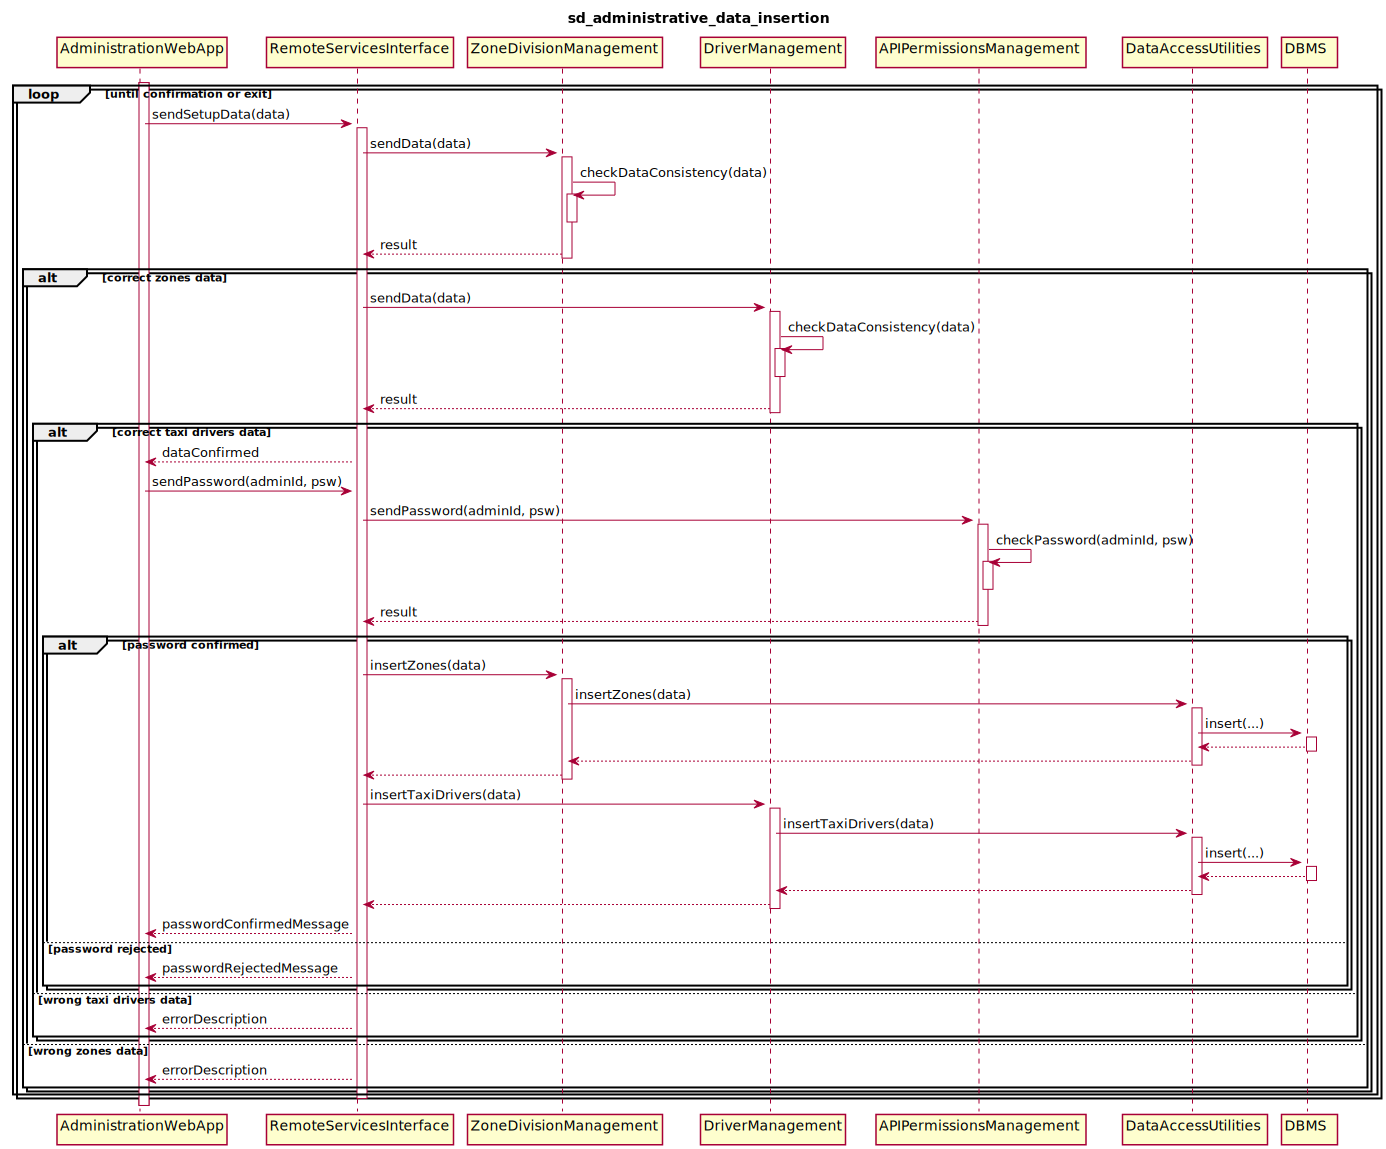
\includepdf[scale=0.95,angle=90]{pdfs/sequence/sd_administrative_data_insertion.pdf}
\end{landscape}

\begin{landscape}
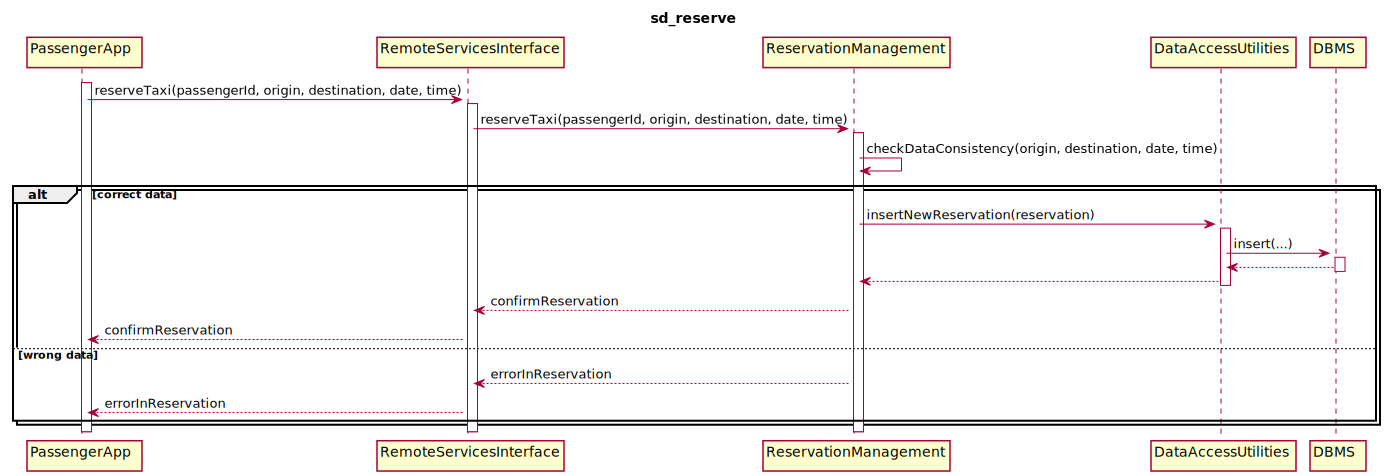
\includepdf[scale=0.95,angle=90]{pdfs/sequence/sd_reserve.pdf}
\end{landscape}

\begin{landscape}
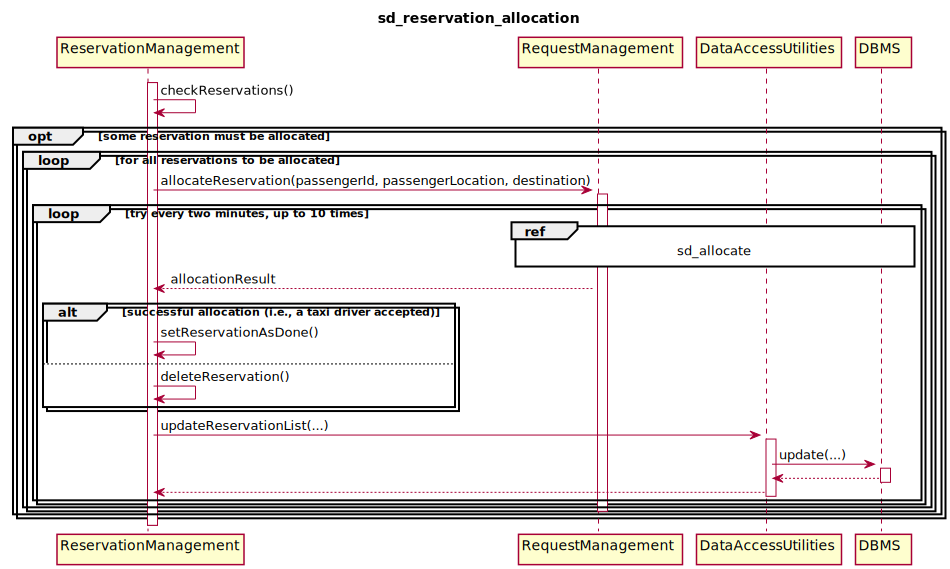
\includepdf[scale=0.95,angle=90]{pdfs/sequence/sd_reservation_allocation.pdf}
\end{landscape}

\begin{landscape}
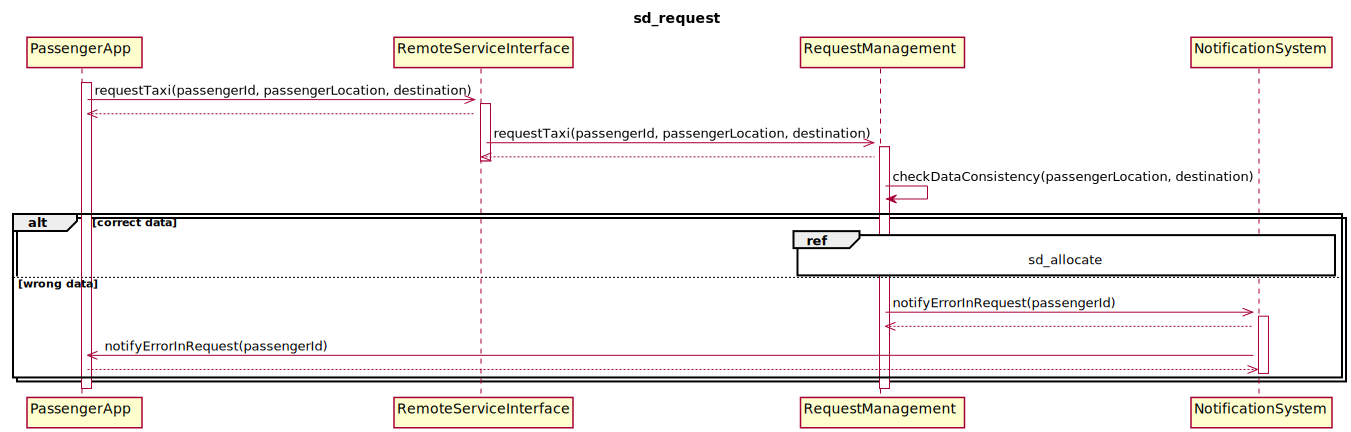
\includepdf[scale=0.95,angle=90]{pdfs/sequence/sd_request.pdf}
\end{landscape}

\begin{landscape}
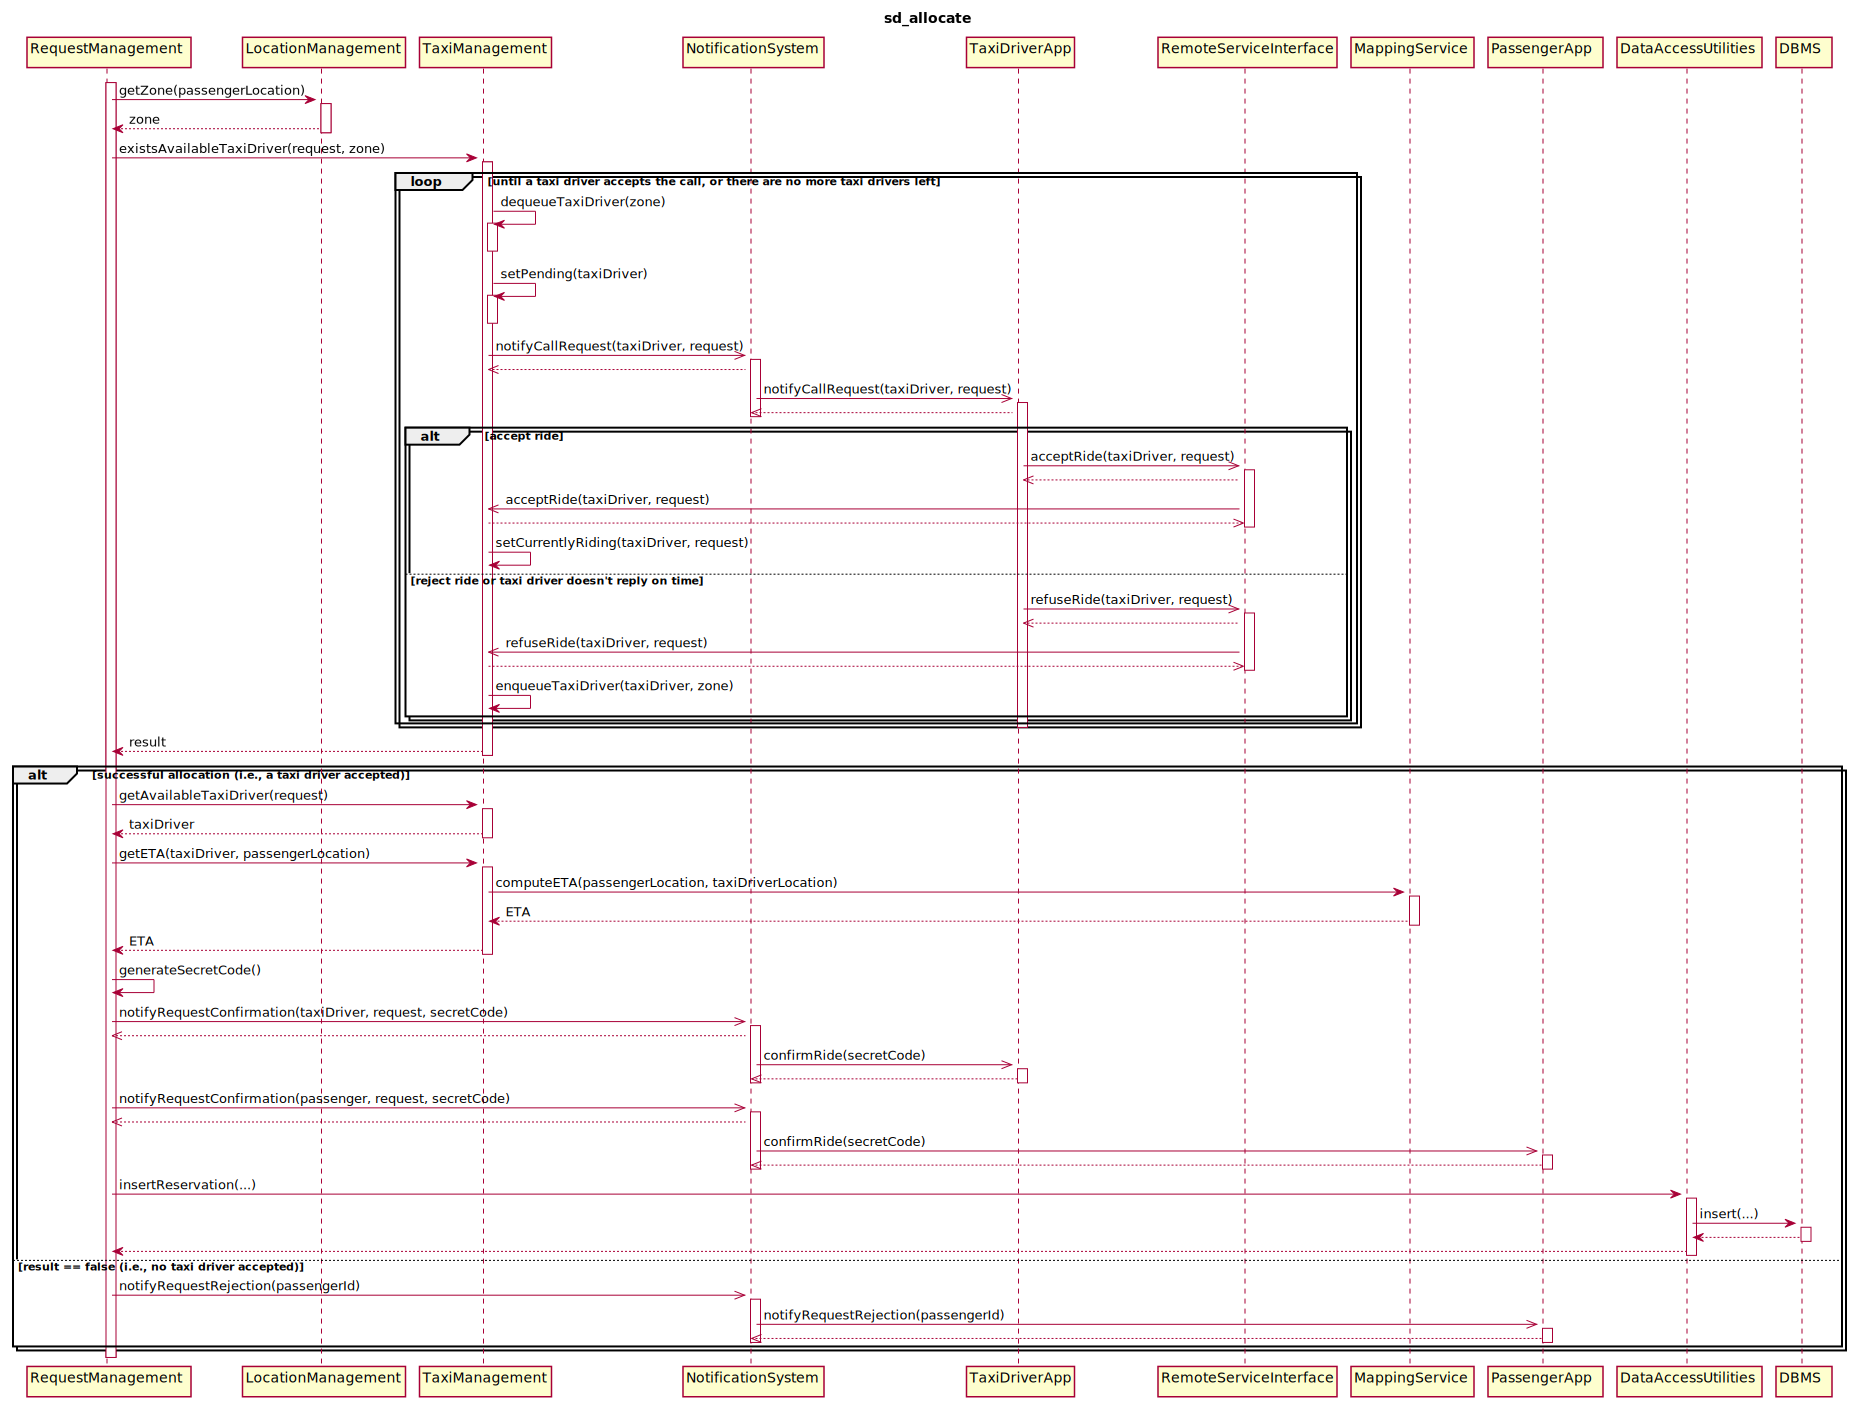
\includepdf[scale=0.95,angle=90]{pdfs/sequence/sd_allocate.pdf}
\end{landscape}

\begin{landscape}
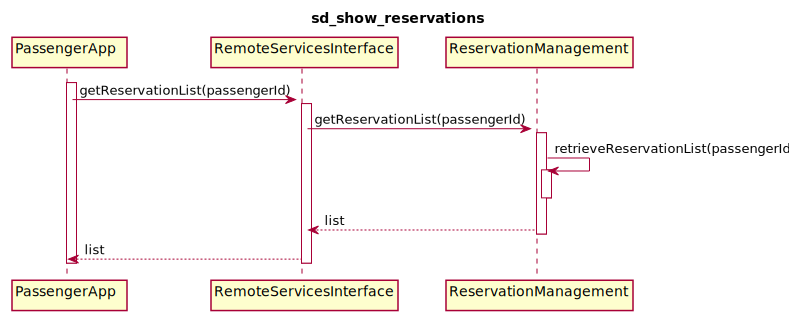
\includepdf[scale=0.95,angle=90]{pdfs/sequence/sd_show_reservations.pdf}
\end{landscape}

\begin{landscape}
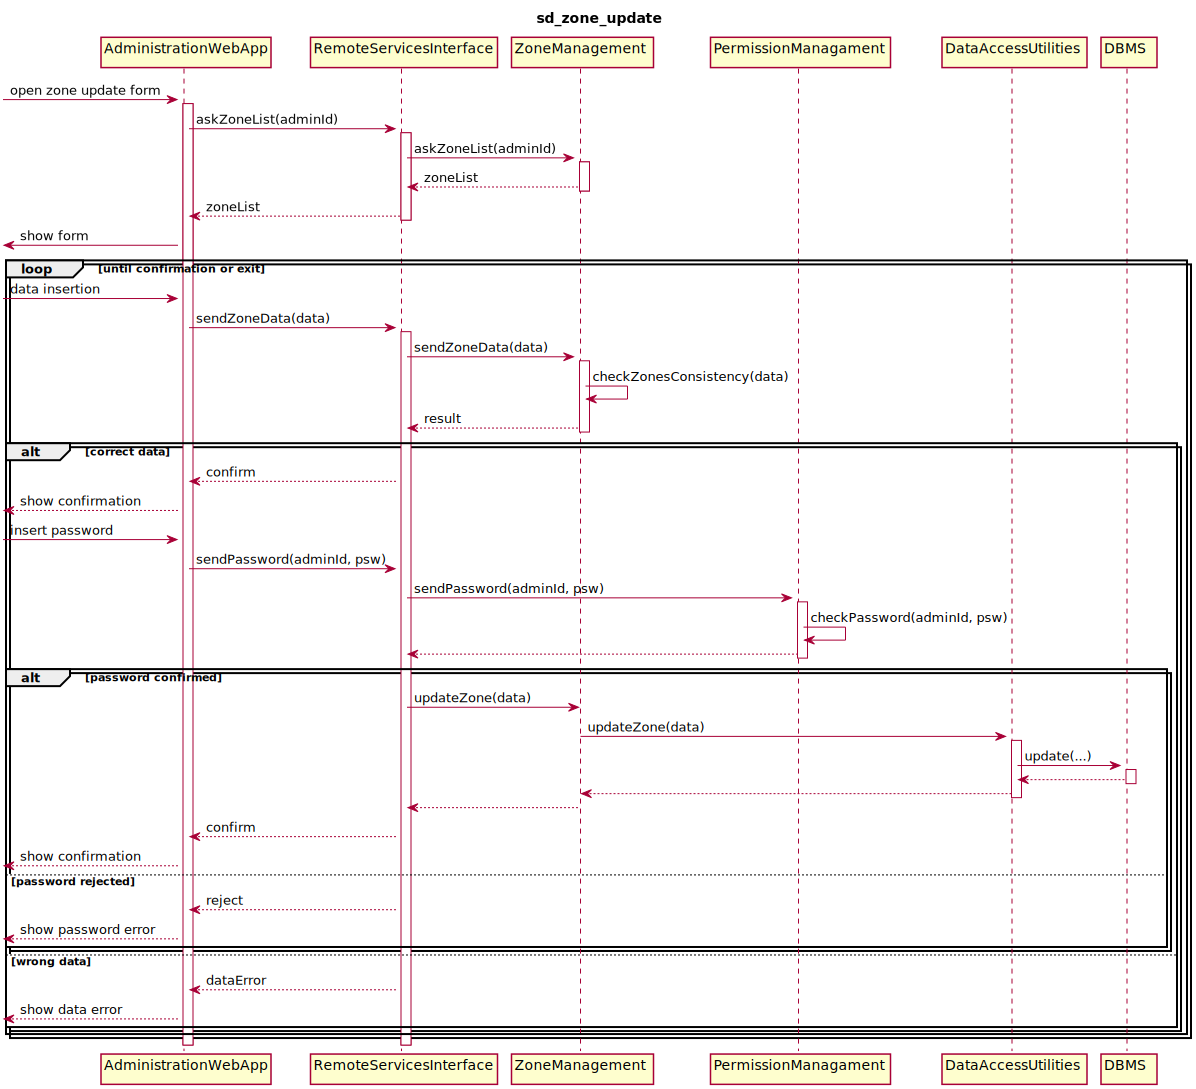
\includepdf[scale=0.95,angle=90]{pdfs/sequence/sd_zone_update.pdf}
\end{landscape}

\begin{landscape}
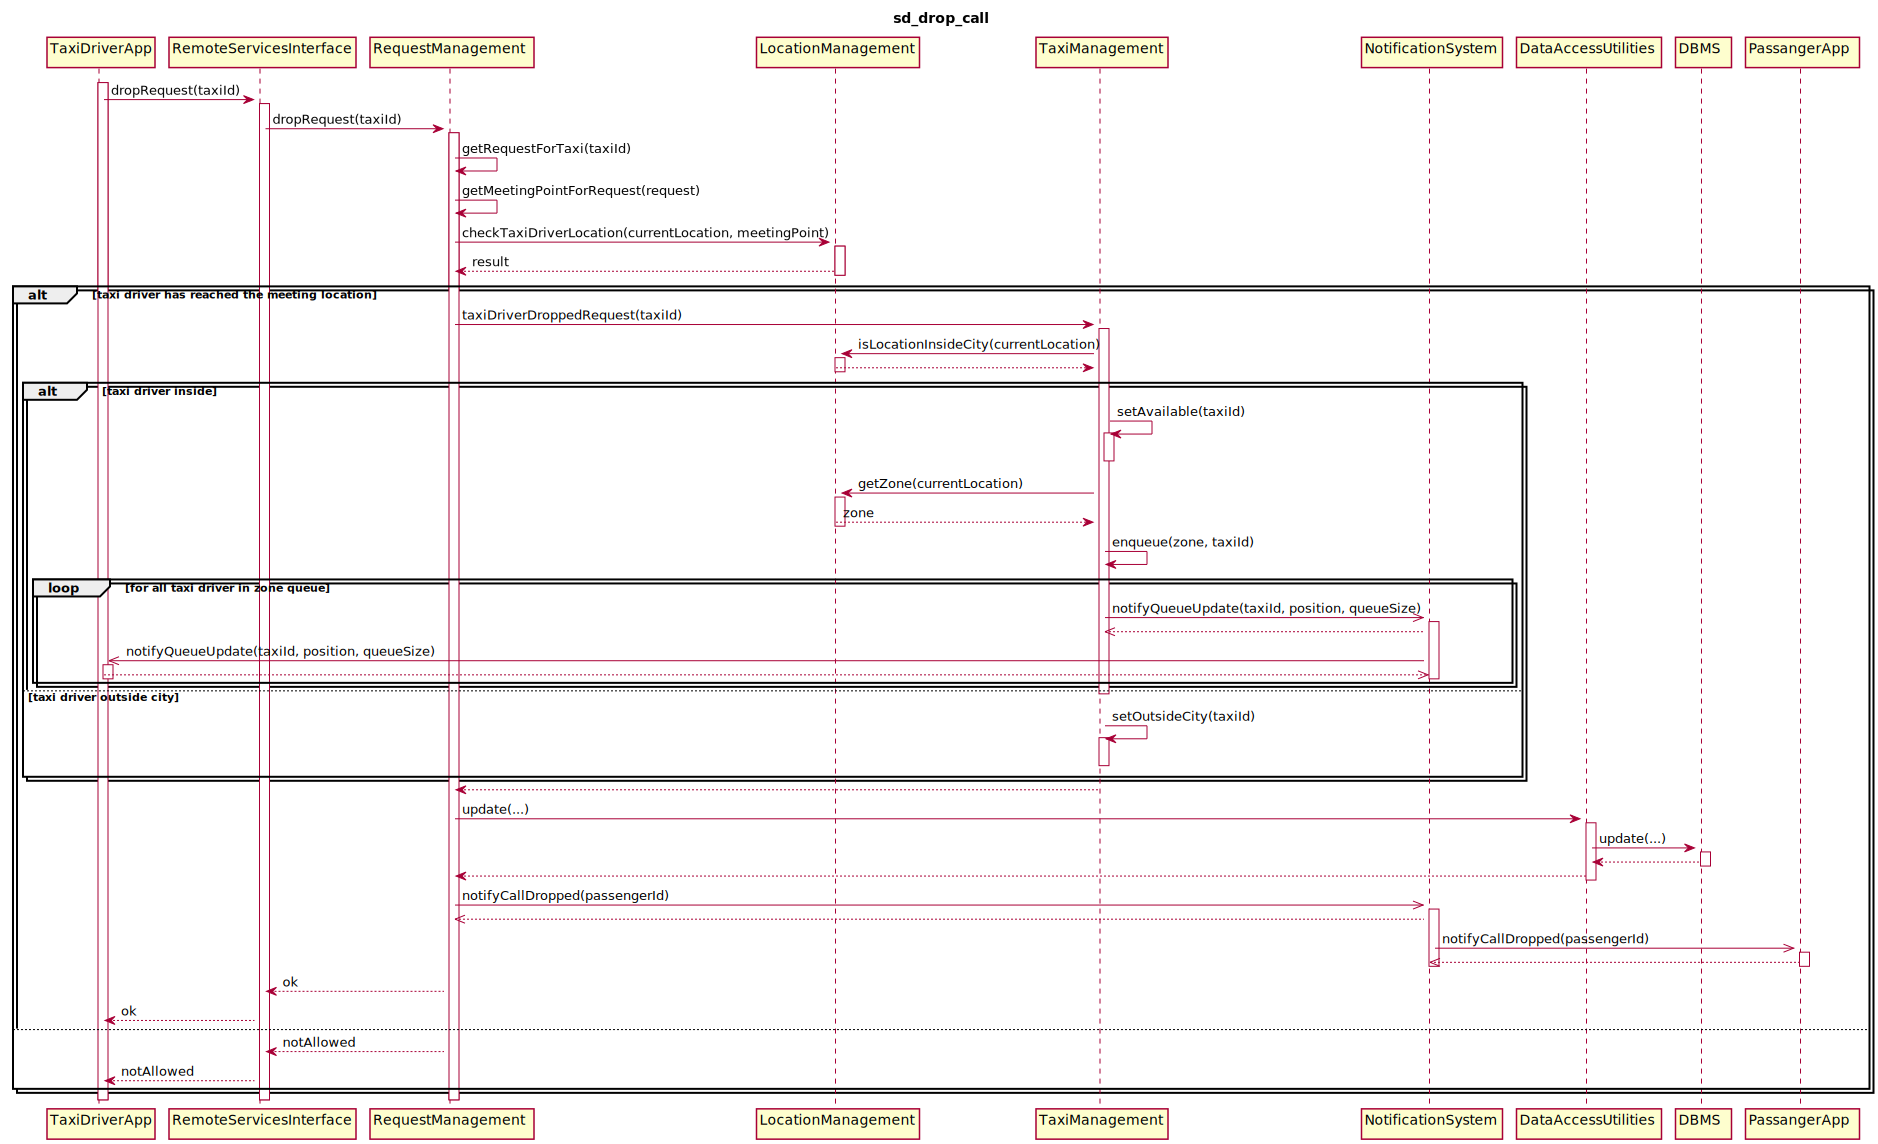
\includepdf[scale=0.95,angle=90]{pdfs/sequence/sd_drop_call.pdf}
\end{landscape}

\begin{landscape}
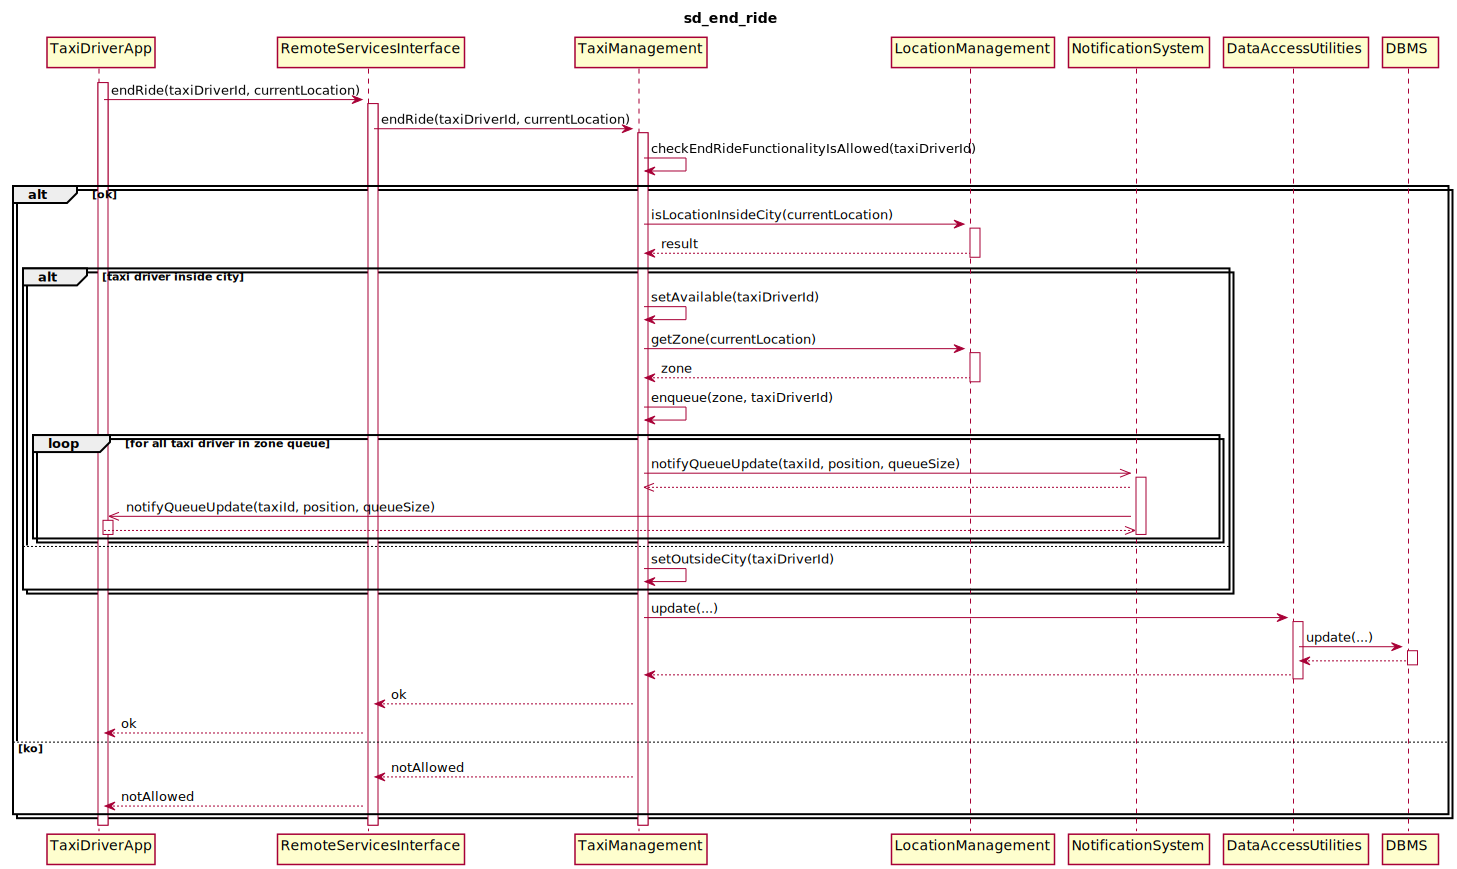
\includepdf[scale=0.95,angle=90]{pdfs/sequence/sd_end_ride.pdf}
\end{landscape}

\includepdf[scale=0.95]{pdfs/sequence/sd_taxi_location_changed.pdf}

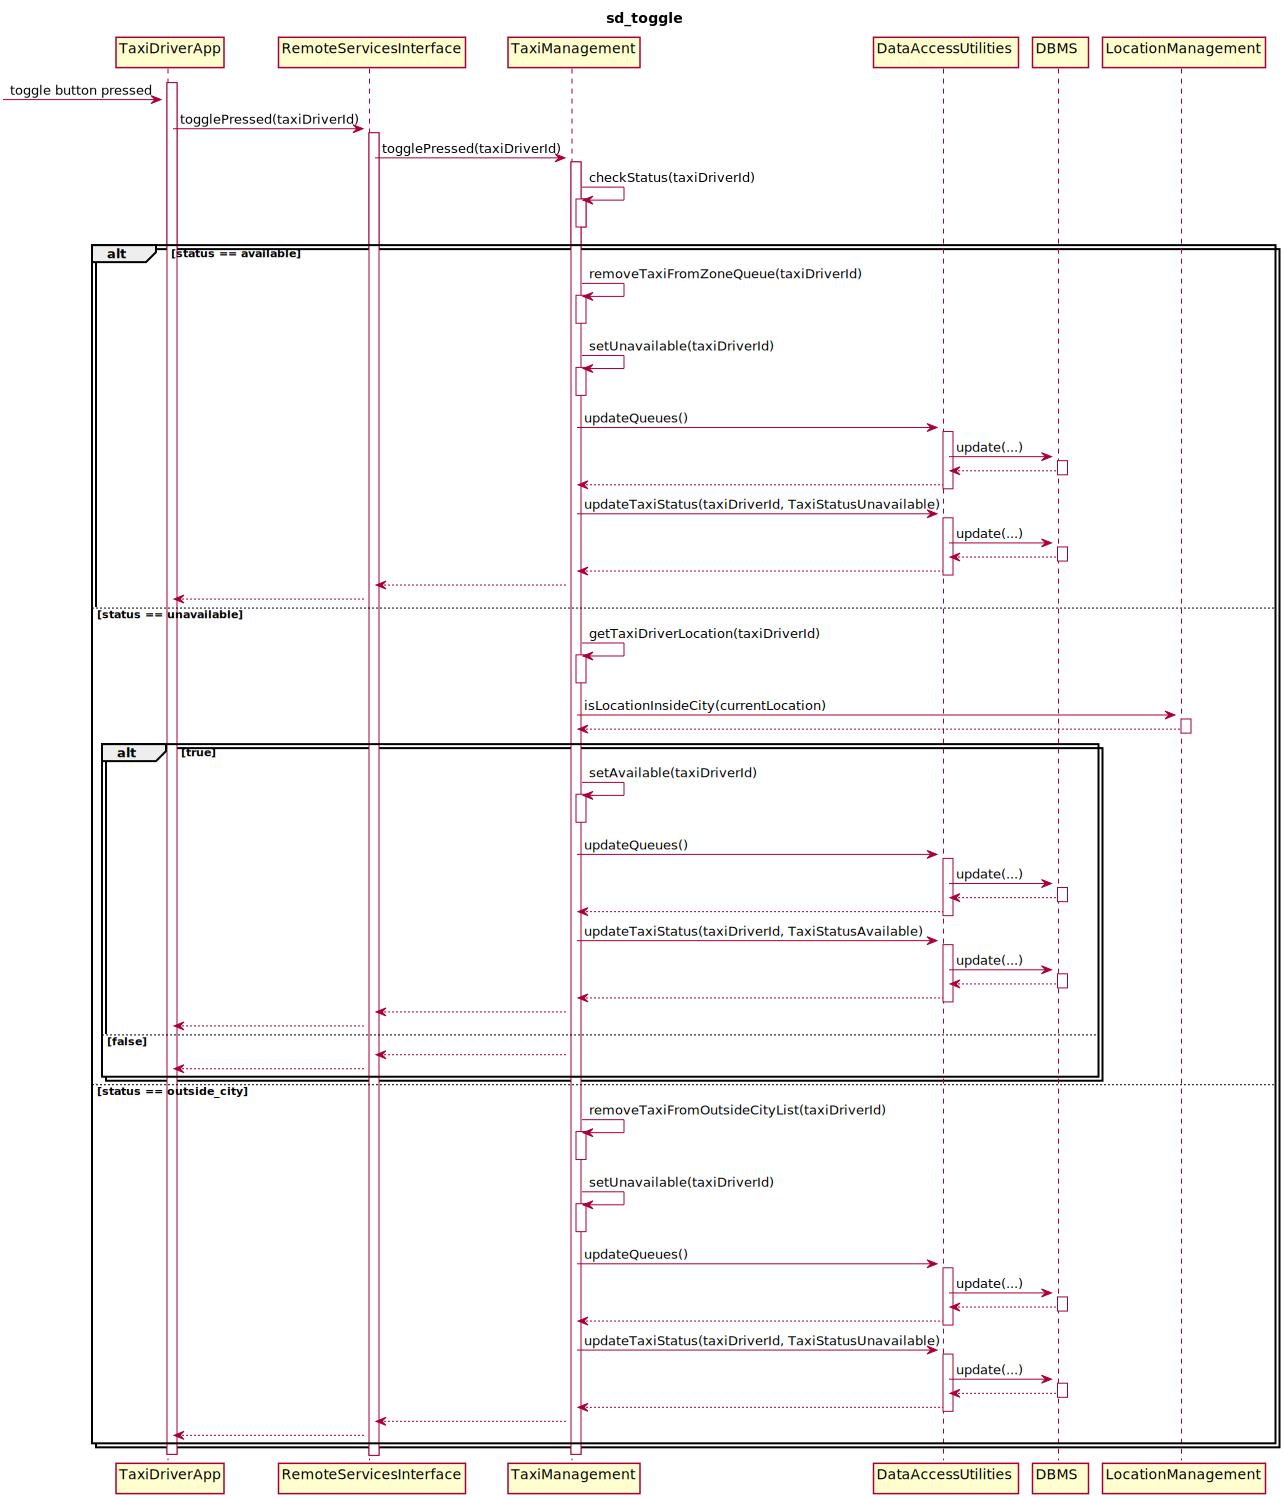
\includepdf[scale=0.95]{pdfs/sequence/sd_toggle.pdf}

\section{Component interfaces}
In this section we're going to describe the interfaces through which the various components of the system communicate. For each interface we'll provide a summary and a description of the main exposed methods. 

It should be noted that, in order to provide a greater level of detail, we will actually distinguish between the various interfaces exposed by each subcomponent of every single component instead of limiting ourselves to the highest level components. 

In the implementation phase, many of these interfaces will actually be further specialized in different classes as needed.
The \textbf{ITaxiManagementSystem} interface is actually an umbrella interface which covers the following different sub-interfaces: 
	\begin{itemize}
	\item The \textbf{IReservationManagement} interface, which represents the way components can interact with the ReservationManagement sub-component. It exposes the following methods:
	\begin{itemize}
	\item reserveTaxi(passengerId, origin, destination, date, time): schedules a new reservation.
	\item getReservationList(passengerId): returns the list of reservations placed by a passenger.
	\end{itemize}
	\item The \textbf{IRequestManagement} interface, which represents the way components can interact with the RequestManagement sub-component. It exposes the following methods:
	\begin{itemize}
	\item dropRequest(taxiId): entry point for requesting a call drop operation.
	\item requestTaxi(passengerId, passengerLocation, destination): implements the necessary operations to request a taxi.
	\end{itemize}
	\item The \textbf{ILocationManagement} interface, which represents the way components can interact with the LocationManagement sub-component. It exposes the following methods:
	\begin{itemize}
	\item checkTaxiDriverLocation(currentLocation, meetingPoint): verifies that the taxi driver has effectively reached both the meeting point.
	\item isLocationInsideCity(location): returns true if the location belongs to the city area, false otherwise.
	\item getZone(location): if the location belongs to the city, returns the zone to which it belongs, otherwise it raises an exception.
	\end{itemize}
	The \textbf{ITaxiManagement} interface, which represents the way components can interact with the TaxiManagement sub-component. It exposes the following methods:
	\begin{itemize}
	\item taxiDriverDroppedRequest(taxiId): verifies if the taxi driver is allowed to drop the request and, if so, performs the necessary operations to drop it.
	\item endRide(taxiId, currentLocation): performs the necessary operations to register that the driver has ended a ride.
	\item acceptRide(taxiDriver, request): registers that the driver has accepted to serve the specified request.
	\item refuseRide(taxiDriver, request): registers that the driver has refused to serve the specified request.
	\item existsAvailableTaxiDriver(request, zone): verifies if there is a taxi driver able to serve the given request and, if so, contacts him and waits for his response; if no taxi driver is available to serve the request, it returns false.
	\item getAvailableTaxiDriver(request): it returns the taxi driver that has been associated to the given request.
	\item getETA(taxiDriver, passengerLocation): returns the estimated time of arrival (ETA) of the taxi driver to the given location.
	\item sendCurrentLocation(taxiId, location): updates the current location of a taxi and performs the necessary update operations to the queues. 
	\item togglePressed(taxiDriverId): updates the availability status of a taxi driver given its previous availability status and the position of the availability toggle.
	\end{itemize}
	\end{itemize}

For the same reason, the \textbf{ISystemAdministration} interface actually comprises many different interfaces, one for each sub-component of System Administration:
\begin{itemize}
	\item The \textbf{IAPIPermissionsManagement} interface, which represents the way components can interact with the API Permissions Management sub-component. It exposes the following methods:
	\begin{itemize}
	\item checkPassword(adminId, password): verifies that the logged in user is an administrator and that the security password to enable the usage of a certain critical functionality is correct.
	\item verifyPermission(appId, operation): verifies that the remote application associated with the appId security token has sufficient privileges to execute the desired operation.
	\end{itemize}
	\item The \textbf{IZoneDivisionManagement} interface, which represents the way components can interact with the Zone Division Management sub-component. It exposes the following methods:
	\begin{itemize}
	\item sendData(data): receives a set of candidate zones that will have to be checked for consistency.
	\item insertZones(data): receives a set of candidate zones that have already been checked for consistency and inserts them inside the database.
	\item updateZones(data): updates the data associated with the specified zones inside the database; if a zone doesn't exist yet it is added, while if a zone is marked as ready for deletion it is removed.
	\item askZoneList(adminId): returns the set of zones stored in the database. 
	\end{itemize}
	\item The \textbf{ITaxiDriverManagement} interface, which represents the way components can interact with the Taxi Driver Management sub-component. It exposes the following methods:
	\begin{itemize}
	\item sendData(data): receives a set of candidate taxi driver data items that will have to be checked for consistency. The actual set of data attributes is described in depth in the RASD.
	\item insertTaxiDrivers(data): receives a set of candidate taxi driver data items that have already been checked for consistency and inserts them inside the database.The actual set of data attributes is described in depth in the RASD.
	\item askDriverList(adminId): returns the set of taxi drivers stored in the database.
	\item updateDrivers(data): updates the data associated with the specified taxi drivers inside the database; if a taxi driver doesn't exist yet it is added, while if a taxi driver is marked as ready for deletion it is removed.
	\end{itemize}
	\item The \textbf{IServiceStatistics} interface, which represents the way components can interact with the Service Statistics sub-component. 
	\item The \textbf{IPluginManagement} interface, which represents the way components can interact with the Plugin Management sub-component. 
\end{itemize}

As for the AccountManagement component, access to its functionalities is made possible by the \textbf{IAccountManagement} interface. Much like previous components, actual operations are carried out using the interfaces exposed by its sub-components, which are the \textbf{IPassengerRegistration}, \textbf{ILogin}, \textbf{IPasswordRetrieval} and \textbf{ISettingsManagement} interfaces. Specific methods for these components haven't been defined at this stage.
Functionalities offered by the Data Access Utilities component are offered through its \textbf{IDataAccess} interface, which exposes a set of methods through which components can easily access the database both for read and write operations. Update, insert, delete and select queries are directly supported and exposed for each kind of key data type; a few examples of these methods can be identified in the sequence diagrams.
The \textbf{INotificationSystem} interface let components request all sort of notification services. In particular, it allows both unicast and multicast notifications via the following methods:
\begin{itemize}
\item notifyCallRequest(taxiDriver, request): notifies a taxi driver that he’s been assigned a request.
\item notifyRequestConfirmation(user, request, secretCode): notifies a user (which can be a taxi driver or a passenger) that the specified request has been successfully handled and gives him the corresponding security code.
\item notifyRequestRejection(passengerId): notifies the passenger that his request has been rejected.
\item notifyCallDropped(passengerId): notifies the passenger that his request has been dropped.
\item notifyErrorInRequest(passengerId): notifies the passenger that his request could not be fulfilled because the required data has been found inconsistent. 
\item notifyZoneChanged(taxiId, newZone): sends a notification to the taxi driver identified by taxiId to alert him that his zone has changed. 
\item notifyExitedCity(taxiId): sends a notification to the taxi driver identified by taxiId to alert him that he has exited the city.
\item notifyEnteredCity(taxiId): sends a notification to the taxi driver identified by taxiId to alert him that he has entered the city.
\item notifyQueueUpdate(taxiId, position, queueSize):  sends a notification to the taxi driver identified by taxiId to alert him that the status of his queue has changed; specifically, it sends him his current position in the queue and the total number of taxis queuing in his zone.
\end{itemize}

Finally, the \textbf{IRemoteServices} interface let remote applications invoke a specific service offered by the central system. In particular, the following methods are exposed: 
\begin{itemize}
	\item sendSetupData(data): receives the initialization data for the system, which is made of tuples containing zone configuration data and taxi drivers data.
	\item sendZoneData(data): receives a set of candidate zones.
	\item sendTaxiData(data): receives a set of candidate taxi drivers.
	\item sendPassword(adminId, password): receives the security password required to perform critical operations and performs the necessary validation procedures.
	\item askZoneList(adminId): returns the list of all stored zones.
	\item acceptRide(taxiDriver, request): notifies the central system that the specified taxiDriver has accepted the specified request.
	\item refuseRide(taxiDriver, request): notifies the central system that the specified taxiDriver has refused the specified request.
	\item dropRequest(taxiId): allows a taxi driver to request a call drop operation.
	\item endRide(taxiDriverId, currentLocation): notifies the central system that the specified taxiDriver has ended his currently assigned ride, and also provides his current location.
	\item requestTaxi(passengerId, passengerLocation, destination): allows a passenger to request a taxi at his current location for a specified destination.
	\item reserveTaxi(passengerId, origin, destination, date, time): allows a passenger to reserve a taxi for a journey going from the specified origin to the specified destination, with pickup scheduled at the given date and time.
	\item getReservationList(passengerId): returns the list of reservations placed by the specified passenger.
	\item sendCurrentLocation(taxiId, location): lets the taxi driver application periodically notify his new coordinates.
	\item togglePressed(taxiDriverId): notifies the central system that the specified taxi driver has switched the availability toggle in his mobile application.
\end{itemize}

\section{Selected architectural styles and patterns}
While designing the software architecture for myTaxiService we looked at all the possible options that enabled us both to satisfy current functional and non-functional requirements and to have enough flexibility for future needs and updates.

In this section we're going to highlight the main architectural styles and patterns that we've decided to use as part of our software architecture, giving a brief description for each of them and explaining why we chose them.

\begin{itemize}
	\item Service Oriented Architecture (SOA). This architectural style allows us to design our system as a set of services which can be separately offered to third parties. The adoption of this architectural style provides several benefits. First, it allows us to easily implement the APIs that must be exposed by the core system, which can be seen as a set of services offered by myTaxiService to remote clients and applications. Second, this give us great flexibility when it comes to further expansions of the set of supported functionalities: by modeling our system as a SOA, it is possible to start offering a set of core services and then increase the number of public APIs as additional components and services are developed. 
	\item Layered Architecture. This architectural style enables a great level of separation of concerns between the various components of the system, such that every component operates at a single logical layer of abstraction. Furthermore, each layer can be separately instantiated on a different machine in a completely orthogonal way, allowing great flexibility in terms of hardware configurations. Finally, this design choice allows us to obtain a greater level of clarity and flexibility: this simplifies the implementation phase, makes testing easier and more effective and dramatically improves maintainability and extendability.
	\item Client/Server Architecture. This architectural style allows us to concentrate all the business logic, which is very computationally intensive, into a number of servers, while the end-user applications only have to offer a limited set of presentation functionalities. It should be noted that we will not use this style with only two tiers, in order to achieve better reliability and availability.
	\item 4-Tier Physical Architecture. This architectural style allows us to run the various components of the system on different devices, not necessarily located in the same server farm. This flexibility in terms of allocation of hardware resources provides a number of key advantages. First of all, it improves security and resilience with respect to attacks: in fact it clearly separates the hardware which runs processes directly connected to the outside world (the web servers) from the hardware running more sensitive and critical services, like the account manager, the administration services and the taxi management system. Furthermore, this gives us the opportunity to easily scale the number of machines of each tier to more efficiently adapt to variations of demand. The tiers that we'll use are: a client tier, a web presentation and remote services tier, a business logic tier and a data tier.
	\item Publish/Subscribe. This architectural style is primarily used in the implementation of the notification system. Even though one-to-one communications between the central system and remotely connected devices could be achieved without the usage of the publish/subscribe architectural style, this design choice provides us greater flexibility with respect to future expansions of the core functionalities. An example of situation in which this architectural style could be useful is the addition of taxi sharing.
\end{itemize}

\section{Other design decisions}
The main infrastructure of the system, which comprises the Remote Services Interface, the Taxi Management System, the System Administration, the Account Management and the Data Access Utilities components will be implemented using the Java Enterprise Edition platform. This design decision has been taken due to the several advantages that this platform has over competing solutions:
\begin{itemize}
	\item It supports multi-tiered applications
	\item It is highly reliable, thanks to its ability to automatically manage multiple instances of the same component
	\item It supports interoperability with different platforms by using SOAP to expose web services to remote clients 
	\item Applications are run inside a managed environment which provides support for reliable database transactions, secure network communications and authentication protocols, thus enabling developers to concentrate their efforts on the peculiar functionalities of myTaxiService
	\item There are many highly efficient and robust application servers which support load balancing
\end{itemize}

As for the mobile applications, we have decided to use the native libraries offered by each mobile platform in order to achieve a better look \& feel and greater performance. This decision comes at the expense of portability of the mobile application code. However, this doesn't actually represent a problem, for three main reasons:
\begin{itemize}
	\item The amount of code contained in each mobile application is extremely small compared to the whole code base of the project, since it's only related to presentation functionalities
	\item All the application logic is already performed on the server and is exposed to mobile applications via standard SOAP web services, which are accessible by any platform without the need to reuse code on the client side
	\item The look \& feel of each platform is peculiar and would require specific libraries to be achieved anyway 
\end{itemize}

The web applications will be implemented using HTML5 technology, in order to be as standard-compliant as possible.

No specific choice has been made as for the DBMS, except for the fact that it will need to be a relational database management system with support for distributed data storage.